\documentclass[aps,pra,preprint,groupedaddress]{revtex4-1}
%\documentclass[aps,prl,preprint,superscriptaddress]{revtex4-1}
%\documentclass[aps,prl,reprint,groupedaddress]{revtex4-1}

\usepackage{graphicx}
\usepackage{amsmath}

% You should use BibTeX and apsrev.bst for references
% Choosing a journal automatically selects the correct APS
% BibTeX style file (bst file), so only uncomment the line
% below if necessary.
%\bibliographystyle{apsrev4-1}

\begin{document}

\title{Phase Dependent Ionization of Rydberg Atoms in Static Fields}

% repeat the \author .. \affiliation  etc. as needed
% \email, \thanks, \homepage, \altaffiliation all apply to the current
% author. Explanatory text should go in the []'s, actual e-mail
% address or url should go in the {}'s for \email and \homepage.
% Please use the appropriate macro foreach each type of information

% \affiliation command applies to all authors since the last
% \affiliation command. The \affiliation command should follow the
% other information
% \affiliation can be followed by \email, \homepage, \thanks as well.
\author{Eric Magnuson}
\email[]{edm5gb@virginia.edu}
\author{Tom Gallagher}
%\homepage[]{Your web page}
%\thanks{}
%\altaffiliation{}
\affiliation{University of Virginia, Department of Physics}

%Collaboration name if desired (requires use of superscriptaddress
%option in \documentclass). \noaffiliation is required (may also be
%used with the \author command).
%\collaboration can be followed by \email, \homepage, \thanks as well.
%\collaboration{}
%\noaffiliation

\date{\today}

\begin{abstract}
Pump-probe schemes using high frequency pulsed light synchronous to strong field low frequency fields are a prolific tool for probing atomic, molecular and surface electron dynamics. We realize one such system in Rydberg states of Li using an 819-nm excitation laser amplutde modulated synchronously to a 15.9-GHz microwave field. We show that when the modulation is at the same frequency of the microwave field, phase dependent ionization is only observed in the presence of static fields. Our results are well described by a computational model. Analysis of this model shows the importance of multiple classical electron orbits.
\end{abstract}

% insert suggested PACS numbers in braces on next line
\pacs{}
% insert suggested keywords - APS authors don't need to do this
%\keywords{}

%\maketitle must follow title, authors, abstract, \pacs, and \keywords
\maketitle

% body of paper here - Use proper section commands
% References should be done using the \cite, \ref, and \label commands
% Put \label in argument of \section for cross-referencing
%\section{\label{}}
%\subsection{}
%\subsubsection{}

\section{\label{sec:intro}Introduction}



Exposing atoms and molecules to a combined near infrared (NIR) laser pulse and the xuv attosecond pulse train (APT) generated from it has proven to be a fruitful probe of ultrafast dynamics in atoms and molecules \cite{Johnsson, Tong, Neidel}. In a typical experiment ionization of an atom or molecule is monitored as the APT is delayed relative to the NIR pulse so that the attosecond pulses coincide with different phases of the NIR field. Since an attosecond  pulse is generated on each half cycle of the NIR field, ionization by the combined NIR and attosecond pulses is equally likely on both half cycles of the NIR field, and the result is a delay dependent ionization signal with a period half the NIR period.

If the process being probed is different for the positive and negative half cycles of the NIR pulse, for example ejection of electrons in a specific direction, the asymmetry cannot be detected by the usual APT, which has a pulse every NIR half cycle. Such an asymmetry can be detected by a single attosecond pulse SAP which samples only one half cycle of the NIR field. Alternatively, such an asymmetry can be observed by using an APT which contains even as well as odd harmonies of the NIR field, which leads to an APT with one pulse per NIR field cycle. This approach has recently been used to observe the directional dissociation of D$_2^+$ \cite{Singhl}. Finally, a process such as ionization can be made asymmetric by combining the NIR pulse with few cycle attosecond pulses in which the strongest first cycle of a cosine pulse has a definite polarity \cite{Kubel}.

The experiments described above are examples of probing dynamics using the combination of a strong low frequency field and a synchronously modulated high frequency field. A different example is exploring the photoionization of atoms in the presence of a strong microwave field by using a visible laser intensity modulated at twice the microwave frequency \cite{Overstreet, Carrat}. As in the NIR-APT experiments, depending upon the phase of the microwave field at which laser excitation occurs, the photoelectron may or may not be ejected from the atom, even if the laser is tuned above the ionization limit. Since neither half cycle of the microwave field is favored, as the modulated laser pulse is delayed relative to the microwave field the ionization signed varies sinusoidally, with half the microwave period, as in the laser experiments described above.

Here we describe an experiment to probe the asymmetric process of laser photoionization of an atom in combined static and microwave fields, both linearly polarized in the same direction. The potential of an atom in a static electric field is shwon schematically in Fig. 1. A laser pulse produces an equal number of photoelectrons leaving the ion core in the uphill and downhill directions, as shown by the double headed arrow in Fig. 1. At one phase of the microwave field all the electrons receive an upfield momentum kick and at the opposite phase they all receive a downhill kick. Since most of the momentum, and energy, transfer occurs during the first half cycle of the microwave field, the final energy of the electron, and whether or not it reamins bound, is very sensitive to the phase of the laser excitation at which laser excitation occurs. To probe this process, which is asymmetric in the two microwave half cycles, we use a visible laser intensity modulated at (not twice) the microwave frequency. We observe the expected modulation in the ionization signal as the modulated laser pulse is delayed relative to the microwave field. As expected the modulation in the ionization signal changes sign when the static field is reversed. Unexpectedly, when the laser is tuned slightly below the limit we observe an unexpected additional reversal of the modulation as the static field is varied.

In the sections which follow we describe the experimental approach, present our observations, describe classical simulations of the process, and make some concluding remarks.


\section{\label{sec:exp} Experimental approach}

Note: \emph{INCLUDE LEVEL DIAGRAM}

Li atoms in a collimated thermal beam pass through a microwave cavity, where they are excited to a high lying Rydberg state or the continuum by three laser pulses, via the route $2s \xrightarrow{\text{671 nm}} 2p \xrightarrow{\text{610 nm}} 3d \xrightarrow{\text{819 nm}} nf, \epsilon f$, as shown by Fig. 2. The 610 nm beam is counterpropagating to the Li beam, and the 670 nm and intensity modulated 819 nm beams cross it at a right angle, forming a 1 mm$^3$ excitation region. This region is at an anti-node of the 15.9 GHz Fabry-Perot microwave cavity. The laser excitation occurs in the presence of a vertically linearly polarized microwave field and a parallel static field, and the $nf, \epsilon f$ photoelectron exchanges energy with the fields as it leaves the Li$^+$ ion core.
% (THIS IS ALL MENTIONED LATER) The 1 mm$^3$ region is much smaller than the extent of the microwave antinode, allowing us to consider the microwave field constant across the region. The interaction region is enclosed on top, bottom and two sides by aluminum plates. Combined with the two Fabry-Perot mirrors, this forms a 10-cm cubic enclosure. Bias voltages can be applied independently to each plate and mirror to control static fields in the interaction region.

The 300 ns long microwave pulse into cavity begins 240 ns before the first laser pulse and ends 20 ns after the last laser pulse. Synchronous with the MW pulse, balanced positive and negative voltage pulses are applied to plates above and below the interaction region to produce a vertical static field in the interaction region. The 20 ns long 610-nm and 671-nm laser pulses are simultaneous and are immediately followed by an 819 nm pulse of 20 ns duration.


One microsecond after the microwave and static fields are turned off we field ionize surviving atoms in Rydberg states within 100 GHz of the ionization limit by applying a negative voltage pulse to the plate below the interaction region. If the static and microwave fields are left on, there are no bound atoms after 1 $\mu$s, and it is for this reason that the fields are turned off. The time delay before the field ionization pulse allows any free electrons produced to disperse. Electrons resulting from field ionization are driven to a microchannel plate (MCP) assembly above the interaction region, and the esulting MCP signal, $S_{Ryd}$, is captured with a gated integrator and recorded in a computer.

\begin{figure}
	\includegraphics[width=0.7\textwidth]{fields}
	\caption{Temporal view of the microwave field (top) phase-locked with the amplitude modulated laser intensity (bottom). The peak laser intensity occurs at the phase $\omega t_0$ of the microwave field, and can be adjusted by an optical delay line.}
	\label{fig:AMLaser}
\end{figure}

The signal of interest is the number of atoms which survive the combined static and microwave fields, in particular its dependence on the phase of the microwave field at which the atoms are excited by the 819 nm laser.
To characterize this phase, or the time delay, we define the microwave field in the cavity as
\begin{equation}
E(t) =E_{mw}\sin{\omega t},
\end{equation}
where $E_{mw}$ is the amplitude of the microwave field, and $\omega$ is the microwave angular frequency. The 819 nm laser intensity $I(t$) is given by
\begin{equation}
I(t) =\frac{I_0}{2}(1+\cos{(\omega (t-t_0)}).
\end{equation}
where $I_0$ is the peak optical intensity, and $t_0$ is the time delay introduced by the delay line. With these definitions $t_0=0$ corresponds to the peak laser intensity's 's occuring at a zero crossing of the microwave field.

To make the measurement we use an optical delay line to delay the modulated 819 nm beam relative to the microwave field in the cavity, as shown in Fig.~\ref{fig:AMLaser}. For each delay$t_0$ we record the signal $S_{Ryd}$ for xxx laser shots and then record a total excitation signal $S_{total}$ for xxx laser shots. The $S_{total}$ signal is obtained by applying the field ionization pulse immediately, cc ns, after the 819 nm laser pulse so as to collect electrons from both bound states and the continuum. Dividing $S_{Ryd}$ by $S_{total}$ yields the normalized signal
\begin{equation}
S=\frac{S_{Ryd}}{S_{total}},
\end{equation}
which is the fraction of laser excited atoms left bound, and $1-S$ is the fraction ionized. All signals reported in this paper are normalized according to Eq.(3).

\subsection{\label{sec:dye} 670 and 610 nm Dye Lasers}

We use two dye lasers at 670-nm and 610-nm to drive the $2s \rightarrow 2p$ and $2p \rightarrow 3d$ transitions, respectively. These dye lasers are pumped by a Quantronix Darwin Nd:YLF laser, which produces 30 mJ, 100-ns (FWHM) pulses at a 1-kHz repetition rate. Using a Pockels cell (PC) and polarizing beam splitter (PBS), the first 20 ns segment of the pulse is picked off and split equally to pump the 670-nm and 610-nm lasers. A second PC and PBS directs the next 20-ns slice, from the peak of the pump pulse, to pump a dye amplifier for the 819-nm laser. The long trailing edge of the pump pulse is dumped.

The 670-nm dye laser has a Littman-style cavity and LDS-698 laser dye dissolved in ethanol as a lasing medium \cite{Littman}. The 610-nm laser has a H{\"a}nsch style cavity with Rhodamine-610 laser dye dissolved in ethanol \cite{Hansch}. Both lasers have linewidths (FWHM) of 10-GHz. To minimize unintended ionization from the $3d$ state, both lasers are attenuated to 2 $\mu J$ pulses before being directed to the vacuum chamber.

\subsection{\label{sec:ampmod} Intensity Modulated 819 nm Laser}

\begin{figure}
	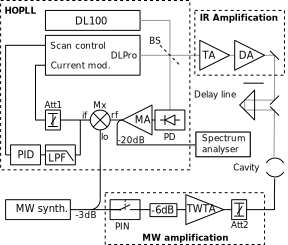
\includegraphics[width=0.7\textwidth]{beatexp}
	\caption{Schematic showing how the amplitude modulated laser is produced, locked to the microwave frequency, and how both the laser and microwave fields are delivered to the interaction region. The AM IR laser is generated by overlapping the DL-Pro and DL-100 laser beams on a beamsplitter (BS). One output is amplified and sent to the interaction region. The microwave field is generated by a synthesizer, formed into pulses by the PIN switch and amplified by the Traveling Wave Tube Amplifier (TWTA) before injection into the microwave cavity. The locking of the IR intensity envelope to the microwave field is performed by the Heterodyne Optical Phase Locked Loop (HOPPL).}
	\label{fig:pll}
\end{figure}

The 819-nm beam is produced using two external-cavity diode lasers, Toptica DL-100 and DL-Pro lasers. The lasers are tuned such that their frequencies are separated by the 15.9 GHz microwave frequency, and the two beams are overlapped on a 50:50 beamsplitter (BS) to produce the intensity modulated beam. As shown by Fig. 4, one output from the beamsplitter is directed to a high speed photodetector to detect the microwave frequency beat note and deliver the signal to a phase-locked-loop. The second output of the 50:50 beamsplitter provides 30 mW of intensity modulated light, which is passed through a tapered amplifier and a dye amplifier. The Toptica Tapered Amplifier increases the continuous beam power to 800 mW. The dye amplifier is pumped by the 20-ns square pulse picked from the peak of the Nd:YLF laser pulse. We use LDS-819 dissolved in ethanol as the amplification medium. The final result is a 20 ns long, 6 $\mu$J pulse of sinusoidally intensity modulated 819-nm light, which is sent to the interaction region. Although the 819 nm beam is produced by two diode lasers, we shall refer to this arrangement as the 819 nm laser.

The intensity modulation of the laser is locked to the microwave frequency with a heterodyne optical phase-locked-loop (HOPLL). The locking is driven by a "fast" feedback to the current input of the DL-Pro, and a "slow" feedback to its scan input. To produce an error signal, the beat note from the photodiode is amplified and mixed with the output of the microwave source. The error signal is passed through a variable attenuator and then connected to the Current input of the Toptica DL-100, providing a lock between the laser intensity modulation frequency and the microwave field that lasts for several minutes.

To achieve longer lock times, on the order of hours, we use a Toptica PID-110 servo unit to drive the scan input of the DL-Pro. The "fast" current lock described above is primarily lost due to the lasers' drifting out of the range that the DL-100 current input can correct. Low-frequency components of the error signal are processed through the PID-110 and fed to the Scan input, which corrects long term drifts in the modulation frequency, leaving only high-frequency errors for the "fast" loop to correct.The phase lock is robust, typically lasting more than xx hours.



Once locked, the phase of the intensity modulation at the BS is constant relative to the MW phase, and its phase relative to the microwave field in the interaction region is controlled by the delay $t_0$ introduced by the optical delay line, which consists of a retro-reflector mounted on a translation stage, as shown in Fig. 4. Using it we are able to extend the path length of the modulated laser beam by several MW wavelengths.

\subsection{\label{cavity} Microwave Apparatus}

A Hittite HMC T-2100 synthesizer tuned to the 15.9-GHz resonance of the microwave cavity is our microwave source. It produces 9 dBm (8 mW) of power, and a splitter diverts half of the power to the microwave mixer to generate the error signal for the PLL. The other half of the signal is formed into 300-ns pulses by a microwave switch, and then amplified by a Hughes 8020H04F traveling-wave-tube-amplifier (TWTA). Between the TWTA and the cavity, there is a 0 to 50 dB variable attenuator, allowing us to control the intensity of the pulse incident on the microwave cavity.

The microwave Fabry-Perot cavity is composed of two brass spherical mirrors. These mirrors have 10 cm radii of curvature, 10.2 cm diameters, and an on axis separation of 7.83 cm. The 15.9 GHz resonance is the TEM$_{008}$ mode of the cavity, with a quality factor $Q=3600$. We are able to determine the field inside the cavity with an uncertainty of 15\%. The 300 ns long microwave pulses are injected into the cavity 280 ns before the end of the last laser pulse and are turned off 20 ns after the end of the laser pulse. When the microwaves are turned off, the microwave field decays with a time constant of vvv ns.

\subsection{\label{fields} Static Fields}

This experiment depends on the detection of long lived Rydberg states close to the ionization limit. To prevent these states from ionizing before detection, we must minimize the ambient static field in the interaction region. We accomplish this by surrounding the interaction region on two sides with the brass microwave cavity mirrors, and on the remaining two sides, top, and bottom with polished aluminum plates. A voltage can be applied independently to each plate or mirror, allowing us to compensate ambient static fields in every direction. We measure the depressed ionization limit (DIL) to minimize stray fields and estimate the residual static field. In this manner, we determine the remaining static field to have a magnitude of 1.5 mV / cm. This results in a DIL of 7 GHz below the the zero field ionization limit. This value for the DIL remained constant for all the experiments discussed in this paper.

To apply a pulsed vertical static field to the interaction region during excitation of Rydberg states we use a two-channel arbitrary waveform generator (AWG) to apply 300-ns square pulses of opposite magnitudes to the top and bottom bias plates. This square pulse is synchronous with the microwave pulse. One microsecond after the final laser pulse, the same AWG applies a -xxV voltage step to the bottom plate to produce a -0.65 V / cm ionization field, ionizing high-lying states and driving the resulting electrons toward the MCP stack.

\section{\label{results} Results}

\begin{figure}
	\includegraphics[width=0.7\textwidth]{phase_delay}
	\caption{Rydberg state signal as the phase delay is scanned. The central laser frequency $2\pi\omega_0$ is tuned to 2 GHz above the DIL. The vertical scale is normalized such that 1 is the total number of electrons excited by the 819 nm laser. When no pulsed field is applied, there is no observed phase modulation. As the pulsed field in increased,  phase dependence in the signal grows and then lessens as the total mean signal decreases. Grey shows the experimental data, while the solid sinusoidal curves trace the best fit to Eq.~\ref{eq:modfit}.}
	\label{fig:phase_delay}
\end{figure}

The delay scans of Fig. 5 show many of the important features of our observations. They are the result of detecting the Rydberg field ionization signal while scanning the time delay $t_0$ with the center frequency of the 819 nm laser tuned 2 GHz above the DIL (5 GHz below the zero-field ionization limit), in the presence of a microwave field of amplitude $E_{mw}=$4 V/cm and several values of the static field. All of the data reported in this paper were taken with this microwave field. Instead of plotting the signals vs the time delay $t_0$ we plot them vs the phase shift $\phi_0=\omega t_0$ of the 819 nm laser intensity envelope relative to the microwave field, as shown by Fig. 3. We do not know the absolute phase $\phi_0$, so we assign the phase $\phi_0=\pi/6$ to the phase at which the maximum number of Rydberg atoms is observed with the laser tuned 2 GHz above the DIL and static field $E_s=$10 mV/cm. All delay scans follow this convention, and all signals are normalized according to Eq. (3).

In Fig. 5 we shown the results obtained $E_{pulse} =$ 0, 7.2, -7.2, 36.0 and 108.0 mV/cm, all in the vertical direction. The results are in accord with our expectations. First, with zero static field, there is no observed phase dependence, while at 7.2 mV/cm there is a 5\% peak to peak (PP) modulation, in agreement with the expectation that a modulation at the microwave frequency ionization can only be observed when a static field is applied in addition to the microwave field. Equally important, when the static field is reversed, to -7.2 mV/cm, the phase dependent modulation reverses sign, as shown by Fig. 3. As $E_s$ is increased further, both the mean signal and the peak to peak modulation decrease, and the delay at which the detected signal is greatest shifts somewhat at higher pulsed field,

While the addition of a static field in the z direction breaks the symmetry of the two microwave half cycles, a horizontal field should not, and in Fig. 6 we show delay scans analogous to those in Fig. 5. In this case the laser is tuned 14 GHz below the DIL, and the magnitude of the static field is 14 mV/cm. By applying voltages to the bias plates we can apply fields at an angle $\theta$ to the horizontal ($90^{\circ}-\theta$ from the z axis). As shown in Fig. 6, there is no modulation with with a horizontal static field, and the observed modulation changes sign as the static field is rotated from having a positive to negative z component.

With the laser tuned 2 GHz above the DIL we have taken extensive data, of which those shown in Fig. 5 are representative. To present these data in a more compact way we quantify them by fitting the observed phase scans to the sinusoidal form:
\begin{equation} \label{eq:modfit}
S = S_m  \cos{[ \phi_0-\pi/6]} + S_0,
\end{equation}
where $S_0$ is the phase average signal, and $S_m$ is the amplitude of the modulation. We constrain $\phi_0$ to lie in the range $0\leq \phi_0\leq \pi$, which results in the plots shown in Fig. 6. As expected, $S_0$ decreases from $S_0)=0.3$  as the magnitude of the static field is increased. the amplitude of the modulation $S_m$ is an odd function of the static field, reaching its maximal positive and negative values at $E_s=\pm 10$mV/cm. Finally, the phase $\phi_0$ is approximately constant.

When the 819 nm laser is tuned 14 GHz below the DIL, the average number of surviving atoms increases, as shown by Fig. 7, which is expected. Unexpectedly, with this laser tuning a small static field results in a modulation of opposite polarity to that seen in Fig. 6. As the amplitude of the static field is raised, the modulation changes sign, and at static fields larger than $\pm25$ mV/cm it has the same sign as seen in Fig. 6. While the sign reversal relative to Fig. 6 at small static fields is surprising, the similarity at higher static fields is not.


 

\begin{figure}
	\includegraphics[width=0.7\textwidth]{circle_static}
	\caption{With the central IR frequency $2\pi\omega_o$ tuned to 14 GHz below the DIL, the angle above the horizontal of a 14.4 mV/cm pulsed field is rotated by applying pulsed voltages to vertical and horizontal bias plates. When the pulsed field is perpendicular to the vertical MW and IR polarization, there no phase dependence. The phase dependence grows as $\vec{E}_{pulsed}$ is rotated to have a larger vertical component. The measurement is repeated in three sets, and linear regression on the combined data set shows the peak to peak modulation crosses zero at $6.0 \pm 0.9$ degrees. This corresponds to $\vec{E}_{pulsed} \cdot \hat{z} = 1.5 \pm 0.2$ mV/cm, which is the approximate size of our stray static field.}
	\label{fig:CircleStatic}
\end{figure}



\begin{figure}
	\includegraphics[width=0.5\textwidth]{ModvsField}
	\caption{Mean signal ($S_0$) and peak-to-peak modulation ($2\cdot A$) against applied pulsed static field for excitation laser central frequencies of +2 GHz, -14 GHz, and -30 GHz relative to the DIL. A negative peak-to-peak modulation indicates the greatest Rydberg signal is detected with an optical delay near $\omega t_o = 7\pi/6$, while a negative modulation indicates the detected signal is greatest near $\omega t_o = \pi/6$.}
	\label{fig:ModvsField}
\end{figure}

Finally, Fig.~\ref{fig:ModvsField} shows the results for the laser tuned to DIL - 30 GHz. They resemble the DIL - 14 GHz case of Fig.~\ref{fig:ModvsField} (b), except that there is no modulation for a finite field range, -20 mV/cm $<E_s<$ 20 mV/cm, around zero static field. The appearance of this new feature is due to the fact that the presence of a small static field plays a diminishing role as the laser is tuned progressively further below the limit. As a result, it is not surprising that for small static fields we obtain the zero field result.

\section{\label{sec:disc} Comparison to Computational Model}

To understand the results presented in Fig.~\ref{fig:ModvsField}, we conducted two classical computational models.  First, we used a 1 dimensional model to calculate the fate of an $e^-$ after it's first orbit. Energy exchange with the MW field occurs only over the first-half-cycle very close to the atom core. The long orbit of an $e^-$ in the pulsed field and Coulomb potential is unaffected over time periods greater than one cycle. As such, we can calculate what happens to an $e^-$ in this first orbit as a function of $E_{pulse}$ and the orbital energy $e^-$ has after energy exchange with the MW field: $W_{orbit} = W_0 + \Delta W_{MW}(\omega t_0)$.

\emph{ADD MATH DESCRIPTION OF TURNING AND BINDING TIMES HERE.}

The results of this calculation for uphill and downhill $e^-$ are shown in Fig.~\ref{fig:orbits}. For uphill electrons, there are four qualitatively distinct behaviors. Deeply bound electrons and orbits in strong pulsed fields are in region (d). These electrons are launched uphill against the combined Coulomb and pulsed field potential and execute an orbit that returns to the core before 20 ns. With the MW field still on, the $e^-$ will again exchange energy with the MW field, and execute another orbit. Because orbit times are much larger than the MW period, the phase of the phase of the MW field is essentially random when the $e^-$ returns, and $e^-$s will undergo a random walk in energy over many orbits. As such, whether $e^-$s in this region ionize is probabilistic. The deeper below the ionization limit this random walk starts, the less likely ionization is to occur.

\emph{QUICK NOTES, NEED TO FLUSH OUT}

In regions (a) and (c), the $e-$ undergoes a long orbit and does not return to the core before the pulsed field shuts off at 20 ns. When the $E_{pulsed}$ shuts off, the $e^-$ is left with a positive energy $W = v^2/2 - 1/r$, and will ionize. Region (b) is a narrow exception, where the field shuts off very near the apoaxis of the $e^-$ orbit, and it is left in a very long period bound state, and will remain bound.

Similar behaviors are shown in the downhill case. $e^-$ in region (d) below the depressed potential barrier will return to the core before 20ns and undergo a random energy walk. Above this in region (a) the electron will directly ionize. There is again a small region (b) where the field turns off at the apoaxis and the $e^-$ is deposited into a bound, long-period orbit.

Regions (a), (c), and (d) describe the behavior seen in Fig~\ref{fig:ModvsField}. In both uphill and downhill cases, remaining bound is more likely if energy is lost to the MW field. This occurs at $\omega t_0 = \pi/6$ for uphill $e^-$ and $\omega t_0 = 7\pi/6$ for downhill $e^-$. High energy either puts the $e^-$ into region (a) or (c) where it will ionize, while low energy puts the $e^-$ starting as far away from the ionization limit for it's random energy walk in region (d).

For above or at the the ionization limit, a small increase in static field will cause a large drop in downhill signal, while uphill $e^-$ are effected by much larger fields. This leaves the phase dependence of the uphill signal to dominate. This is shown in Fig.~\ref{fig:2DW0}.

Fig.~\ref{2DW20} shows the model at $W_0 = -20$ GHz. Below the ionization limit, a small increase in static field brings the depressed potential barrier seen by downhill electrons closer to $W_0$. As such, the mean downhill signal falls, but the peak to peak modulation increases. This leads to the total phase dependence at small fields being $\pi$ out of phase with the small signal phase dependence when $W_0 = 0$ GHz.

However, as the field increases, the depressed potential barrier moves below $W_0$, and at large fields the downhill signal again disappears. This leaves the uphill electron signal to dominate the total observed signal. This phase dependence is then in phase with the large field signal at $W_0 = 0$ GHz.

\begin{figure}
	\includegraphics[width=\textwidth]{up_and_down_orbits}
	\caption{The fate of an electron after it's first orbit. The y-axis is the $e^-$ orbital energy $W_{orbit} = W_0 + \Delta W_{MW}$ after exchanging energy with the MW field, and the x-axis shows the strength of $E_{pulsed}$. \textbf{Uphill Electrons:} \textbf{(a)} High energy $e^-$ in low field will directly ionize. \textbf{(b)} $E_{pulse}$ shuts off near the apoapsis of the $e^-$ orbit, and is left in a bound long-period orbit. \textbf{(c)} $E_{pulse}$ shuts off as the $e^-$ is returning to the core with positive orbital energy. It will swing around the core as the MW field rings down and ionize. \textbf{(d)} Low energy $e^-$ in high field orbits return to the core before $E_{pulse}$ or $E_{MW}$ turn off at 20 ns. The electron exchanges energy with the MW field at every return to the core, resulting in a random walk in energy that may result in ionization or remaining bound. \textbf{Downhill Electrons:} \textbf{(a)} High energy $e^-$ in small field will directly ionize. \textbf{(b)} At 20 ns the $e^-$ is near it's apoaxis and will be left in a long-period bound orbit. \textbf{(d)} The $e^-$ returns to the core before 20 ns and undergoes a random energy walk. Whether the final state is bound after many orbits is probabilistic.}
	\label{fig:orbits}	
\end{figure}

\begin{figure}
	\includegraphics{W0_2D}
	\caption{Calculated observed signal from our 2 dimensional model, with initial energy $W_0 = 0 GHz$. The contributions from uphill and downhill electrons are in orange and blue, respectively, with the total expected signal in Green. At $E_{pulse} = 0$ mV/cm, uphill and downhill signals have opposite phase dependence, resulting in a flat total signal. As signal increases, downhill $e^-$ at every launch phase all ionize, and the total signal is dominated by the uphill signal.}
	\label{fig:2DW0}
\end{figure}

\begin{figure}
	\includegraphics{W20_2D}
	\caption{Calculated observed signal from our 2 dimensional model, with initial energy $W_0 = -20 GHz$. Uphill and downhill signals are in blue and orange, respectively, with total signal in green. As in Fig.~\ref{fig:2DW0}, at $E_{pulse} = 0$ mV/cm, the uphill and downhill signals result in a flat total signal. At $E_{pulse} = 7.2$ mV/cm, the downhill signal is diminished, but the total phase dependence increases. The total signal shows a phase dependence shifted by $\pi$ from the small field signal for $W_0 = 0 GHz$ in Fig.~\ref{fig:2DW0}. At $E_{pulse} = 100$ mV/cm, downhill $e^-$ almost all ionize, and the uphill signal dominates the total signal.}
	\label{fig:2DW20}
\end{figure}

\section{\label{sec:conc} Conclusions}

\emph{EMPTY}

%\bibliography{basename of .bib file}

\end{document} 